\capitolo{LAMG: Lean Algebraic MultiGrid}
\label{cap:LAMG}

Quella del \emph{multigrid algebrico} (AMG) è una classe di risolutori di sistemi lineari che trae le sue origini negli anni '80 ed ancora sotto attivo sviluppo.
Questi metodi si dividono in due fasi principali.\\
Nella prima, detta di \emph{setup}, viene costruita una gerarchia di matrici sempre più coarse, cioè di dimensioni minori, senza utilizzare informazioni geometriche deducibili dall'istanza di problema, come invece avviene nei metodi del \emph{multigrid geometrico}.\\
Nella seconda fase, detta di \emph{solve}, si effettuano dei cicli multigrid come quelli descritti nell'algoritmo~\vref{alg:MGM}.

LAMG è un algoritmo di tipo AMG che risolve sistemi di equazioni lineari della forma
\begin{equation*}
Ax = b
\end{equation*}
dove la matrice dei coefficienti $A$ è una matrice laplaciana di grafo.
Può trovare quindi applicazione come metodo iterativo nella risoluzione dei sistemi nella forma~\eqref{eqn:IP} legati ai problemi di MCF e, più in generale per la risoluzione di problemi di grafo.\\
Sia dato un grafo $G=(\N,\E,\w)$, dove $\N$ è un insieme di nodi, $\E$ un insieme di archi e $\w$ la funzione che assegna un peso positivo a ciascuno degli archi di $\E$. \\
Definiamo la matrice diagonale $D$ avente come elementi diagonali la somma dei pesi degli archi di ciascun nodo
\begin{equation}
d_i = \sum_{j \in \N,\,j \ne i} \w_{i,j} \quad \forall i \in \N
\end{equation}
Definiamo inoltre la matrice di adiacenza pesata del grafo $G$ come
\begin{equation}
a_{i,j} = 
\begin{cases}
\w_{i,j} & \text{se } (i,j) \in \E\\
0 							& \text{altrimenti}
\end{cases}
\end{equation}
La matrice Laplaciana di grafo è data da
\begin{equation}
L = D - A
\end{equation}
Tale matrice è simmetrica e a predominanza diagonale.
\sezione{Le scelte di LAMG}
Nel capitolo~\vref{intro} si è visto come ciascuna implementazione multigrid debba effettuare principalmente due scelte:
\begin{itemize}
\item Scegliere il metodo iterativo da utilizzare come smoother
\item Scegliere che tipo di operatore di restringimento utilizzare per poter proiettare il residuo dallo spazio $\Omega_n$ al sottospazio $\Omega_k$
\end{itemize}

La scelta del primo ricade sul metodo di Gauss-Seidel poiché richiede meno memoria rispetto, ad esempio, al metodo di Jacobi.

Si consideri la decomposizione della matrice $A$ data da
\begin{equation*}
A = D - B - C
\end{equation*}
dove
\begin{equation*}
d_{i,j} =  
\begin{cases}
a_{i,j} & \text{se } i = j\\
0 & \text{se } i \ne j
\end{cases},\,
b_{i,j} =
\begin{cases}
-a_{i,j} & \text{se } i > j\\
0 & \text{se }i \leq j
\end{cases},\,
c_{i,j} =
\begin{cases}
0 & \text{se } i \geq j\\
-a_{i,j} & \text{se } i < j
\end{cases}\end{equation*}

Scegliendo $M = D - B$ e $N = C$ si può riscrivere il sistema di partenza come 
\begin{equation*}
(M- N)x = b
\end{equation*}
ovvero
\begin{equation*}
Mx = Nx + b
\end{equation*}
da cui segue
\begin{equation*}
x = M^{-1}Nx+M^{-1}b
\end{equation*}  

Questo sistema, posto
\begin{equation*}
G = M^{-1}N = (D-B)^{-1}C
\end{equation*}
e scelta una soluzione iniziale $x^{(0)}$, da luogo alla successione
\begin{equation}
\label{eqn:GS}
x^{(k)} = Gx^{(k-1)}+(D-B)^{-1}b
\end{equation}
Per descrivere come viene implementato il metodo di Gauss-Seidel conviene prima trasformare la~\eqref{eqn:GS} così
\begin{equation*}
\begin{split}
(D-B)x^{(k)} &= Cx^{(k-1)} + b\\
Dx^{(k)} &= Bx^{(k)} + Cx^{(k-1)} + b\\
x^{(k)} &= D^{-1}Bx^{(k)}+D^{-1}x^{(k-1)} + D^{-1}b
\end{split}
\end{equation*}

Il metodo di Gauss-Seidel viene allora implementato nel modo seguente
\begin{equation}
x_i^{(k)} = \frac{1}{a_{ii}} \bigg[b_i - \sum_{j=1}^{i-1} a_{ij}x_j^{(k)} - \sum_{j=i+1}^{n} a_{ij}x_j^{(k-1)} \bigg],\, i=1,2,\dots,n
\end{equation}

Il vantaggio fondamentale di questo metodo è che per calcolare le componenti del vettore $x^{(k)}$ si utilizzano anche le componenti già calcolate dello stesso vettore. Quindi è sufficiente disporre di un solo vettore in cui si sostituiscono le componenti via via che vengono calcolate.
Inoltre la convergenza è garantita se applicato alla matrice laplaciana poiché la predominanza diagonale di quest'ultima fornisce una condizione \emph{sufficiente}~\cite[110]{Toporagno}.\\
\\
Per quanto riguarda la seconda scelta LAMG utilizza una combinazione di due metodi per costruire, ad ogni livello, l'operatore di restrizione.

Il primo, detto \emph{Aggregation}, crea la matrice più coarse, cioè diminuisce la dimensione della matrice $A$, aggregando i nodi del livello $\Omega_n$ secondo un criterio di prossimità che prende il nome di \emph{affinity}.\\
\\
Il secondo, detto \emph{Low Degree Elimination}, ha lo scopo di eliminare dal grafo quella parte che non può essere aggregata in maniera efficace dall'altro metodo.
Nella sezione~\vref{subsec:AggeLDE} vedremo nel dettaglio il funzionamento di questi due metodi.

Il sistema del livello più basso $L$ viene risolto utilizzando il metodo di Gauss-Seidel, se la convergenza risulta essere veloce, oppure utilizzando un metodo diretto su un sistema aumentato~\cite{lamg_Report}.

\sezione{Operatori di restringimento di LAMG}
\label{subsec:AggeLDE}

Conforme agli altri metodi multigrid, LAMG costruisce come prima cosa una gerarchia di $L$ sistemi $A_l x_l = b_l$, detti livelli, di dimensioni sempre inferiori rispetto al precedente. Il sistema $A_lx_l = b_l$ corrisponde a quello di partenza. 
Gli altri livelli $i\geq 2$ sono ottenuti con il metodo di Galerkin utilizzando come matrice $R$ o una matrice di eliminazione, e allora il livello corrispondente sarà di \emph{Elimination}, o di aggregazione, e allora il livello sarà di \emph{Aggregation}.
Tali tecniche vengono alternate per la generazione della gerarchia dei livelli.\\
\\
\sottosezione{Low Degree Elimination}
\begin{figure}
\centering
\begin{tabular}{cccc}
\toprule
$|\E_i|$ & $\Delta_m$ & Prima dell'eliminazione & Dopo l'eliminazione \\
\midrule
$1$ & $-1$ & 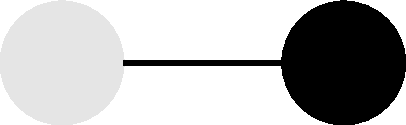
\includegraphics[height=0.015\textheight]{Grafica/el-A} & 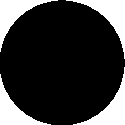
\includegraphics[height=0.015\textheight]{Grafica/el-B}\\
\midrule
$2$ & $-1$ & 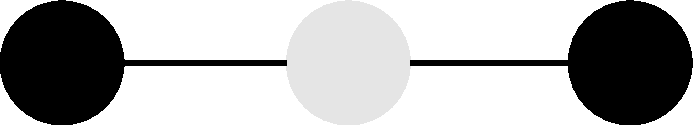
\includegraphics[height=0.015\textheight]{Grafica/el-C} & 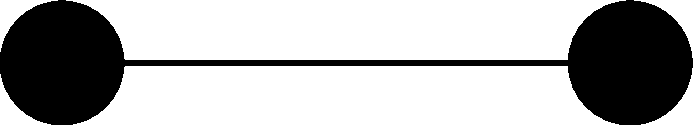
\includegraphics[height=0.015\textheight]{Grafica/el-D}\\
\midrule
$3$ & $0$ & 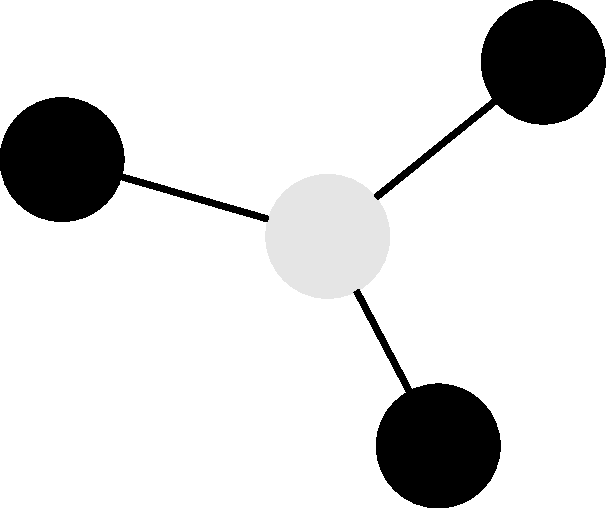
\includegraphics[height=0.04\textheight]{Grafica/el-E} & 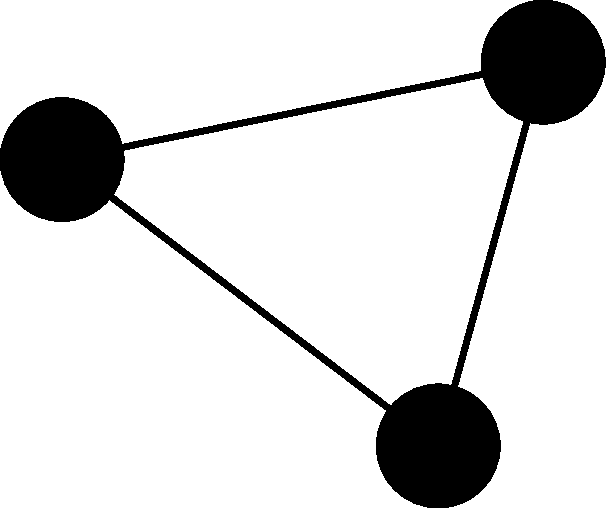
\includegraphics[height=0.04\textheight]{Grafica/el-F}\\
\midrule
$4$ & $+2$ & 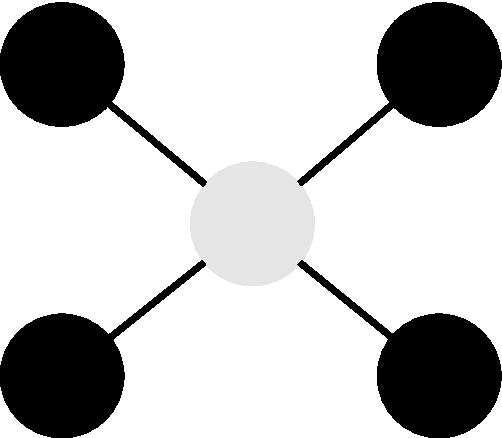
\includegraphics[height=0.04\textheight]{Grafica/el-G} & 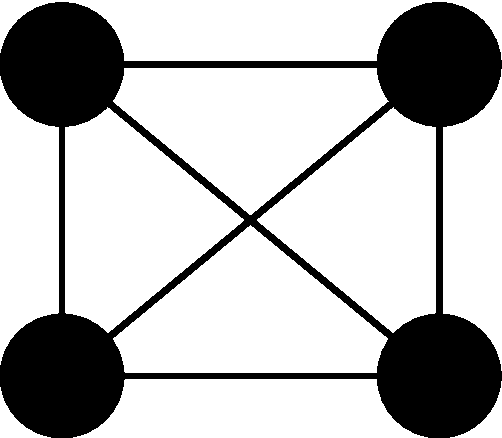
\includegraphics[height=0.04\textheight]{Grafica/el-H}\\
\midrule
\end{tabular}
\caption{Come viene modifica la porzione di grafo interessata prima e dopo l'eliminazione dei nodi candidati (nodi in grigio). $\Delta_m$ è la variazione massima del numero di archi.}
\label{tbl:elimino}
\end{figure}

La creazione di un livello Elimination avviene eliminando dall'insieme dei nodi $\N$ un sottoinsieme $\F$ di nodi indipendenti di grado $|\E_i| \leq 4$.
L'eliminazione di un singolo nodo comporta la connessione di tutti i suoi vicini. 
L'eliminazione di un nodo con grado $|\E_i| \leq 3$ non comporta l'aggiunta di nessun arco, e dunque nessun fill-in per la matrice dei coefficienti, così come riassunto in figura~\vref{tbl:elimino}.
Quando $|\E_i| = 4$, $m$ può aumentare di al più $2$ e questo, nella pratica, è accettabile perché l'alternativa, impraticabile perché costosa, sarebbe quella di monitorare tutti i futuri cambiamenti di $m$ e decidere se eliminare il nodo solo nel caso che questo non comporti maggiori aumenti.
Valori più grandi di $\E_i$ risultano in un impratico fill-in della matrice dei coefficienti.
\\
La selezione dei nodi in $\F$ avviene con una visita su tutti i nodi con grado $|\E_i| \leq 4$. Quando un nodo viene marcato come \textsc{fnode} tutti i suoi vicini vengono marcati come non eleggibili (\textsc{noteliminated}) in modo da garantire l'indipendenza di tale insieme (algoritmo~\vref{alg:LowDegreeNodes}).

Consideriamo ora l'insieme $\C = \N \setminus \F$, cioè l'insieme dei nodi high-degree che rimangono dopo aver eliminato quelli low-degree. Il sistema di partenza $\matr{Ax} = \matr{b}$ si riduce dunque al sistema complementare di Schur definito come

\begin{equation}
\label{eqn:SchurComplementSystem}
A^cx_{\C} = b^c \text{ dove }%
A^c = RAP \text{, }%
b^c = Rb \text{, }%
R  = \Pi (-A_{\F\C}^T A_{\F\F}^{-1},I_{\C})
\end{equation}
dove $\Pi$ è una matrice di permutazione tale che $\Pi^Tx$ mostra tutti i valori dei nodi di $\F$ e poi tutti i valori dei nodi in $\C$.
\eqref{eqn:SchurComplementSystem} è un sistema Laplaciano più piccolo, per il quale vengono eseguiti ulteriori passaggi di eliminazione utilizzando l'algoritmo~\vref{alg:Elimination} fino a quando $\abs{\F}$ non diventa sufficientemente piccolo.

\begin{algorithm}
\caption{$\F = LowDegreeNodes(\matr{A})$}\label{alg:LowDegreeNodes}
\begin{algorithmic}[1]
\State $\N\gets nodes(\matr{A})$, $n \gets size(\matr{A}), \U \gets \Set{u\in\N : 1 \le \abs{\E_u} \le 4}$
\State For each $u \in \U, visited(u) \gets \text{\textsc{notvisited}}$
\For{each $u\in\U$}
	\If{$visited(u) = \text{\textsc{notvisited}}$}
		\If{$\nexists v \in \E_u : visited(v) = \text{\textsc{fnode}}$}\Comment{$u$ può essere eliminato}
			\State $visited(u) \gets \text{\textsc{fnode}}$
			\State For each $v \in \E_u, visited(v) \gets \text{\textsc{noteliminated}}$
		\Else\Comment{$u$ ha un vicino che è in $\F$}
			\State $visited(u)\gets\text{\textsc{noteliminated}}$
		\EndIf
	\EndIf
\EndFor
\State $\text{return } \F = \Set{u \in \U : visited(u) = \text{\textsc{fnode}}}$
\end{algorithmic}
\end{algorithm}

Se nessun nodo viene eliminato in questa fase di eliminazione allora l'attuale livello rimane il coarsest, altrimenti la coppia $(A^c, R)$ definisce il prossimo livello $l+1$.

In entrambi i casi si procede con la fase di aggregazione per tentare di ridurre la dimensione del vecchio livello, o del nuovo appena creato.\\
\\
\begin{algorithm}
\caption{$[\A^c, \Pp, \Q, \Set{\Pp_i,\Q_i}_{i=1}^q] = Elimination(\A)$}\label{alg:Elimination}
\begin{algorithmic}[1]
\State $\A^c \gets \A, \N^c \gets nodes(\A), n_c \gets \abs{\N^c}, \Q \gets \matr{0}_{n_c}, \Pp \gets \matr{I}_{n_c}, q \gets 0$
\While{$n_c > 1$}
	\State $\F \gets LowDegreeNodes(\A^c)$
	\If{ $(\abs{\F} < 0.01n_c)$}
		\State return $[\A^c, \Pp, \Q, \Set{\Pp_i,\Q_i}_{i=1}^q]$
	\EndIf
	\State $q \gets q+1, \C \gets \N \setminus \F$
	\State $\Pie \gets \text{una matrice di permutazione che ordina }\N^c \text{ come } (\F,\C)$
	\State $\Q_i \gets \Pie \cdot \text{diag} \Set{(\A_{\F\F}^c)^{-1},\0_\F },\,\matr{R} \gets (\0_\F, \I_\C)$
	\State $ \Pp_i \gets \Pie \cdot ( -(\A_{\F\C}^c)^T(\A_{\F\F}^c)^{-1},\I_\C)^T$
	\State $\Q \gets \Q + \Pp\Q_i\Rr, \Pp \gets \Pp_i\Pp, \A^c \gets \Pp^T\A^c\Pp, \N^c \gets nodes(\A^c), n_c \gets \abs{\N^c}$
\EndWhile 
\end{algorithmic}
\end{algorithm}

\sottosezione{Aggregation}

Per la creazione efficace di un livello Aggregate è determinante definire quali elementi di $\N$ siano \emph{prossimi}.
I metodi multigrid tipicamente utilizzano misure di prossimità che si basano sui pesi degli archi per operare questa scelta:

\begin{equation}
\label{eqn:ClassicalAMGProximity}
\frac{1 - \abs{\w_{uv}}}{ \max \{ \max_s \abs{\w_{us}} , \max_s \abs{\w_{sv}} \}}
\end{equation}

Questa misura funziona molto bene nel caso si trattino problemi legati alle equazioni differenziali ellittiche alle derivate parziali, dove si possono utilizzare anche informazioni di natura geometrica, ma porta a decisioni di aggregazione infelici nel caso di grafi non locali.

Ad esempio in un grafo a griglia con un arco extra che connette nodi distanti $u$ e $v$ questi rischiano di diventare prossimi e possono essere aggregati (vedi figura~\vref{fig:Agg}a).
A meno che il peso di tale arco non sia molto grande, questo comportamento non è desiderabile perché produce un'aggregazione di nodi che corrispondono a maglie della griglia non correlate tra loro.
Questo è un grande problema poiché i grafi a griglia che compaiono nei problemi GMG discretizzano oggetti reali su cui vogliamo fare simulazioni di fluidodinamica, come ad esempio un alettone della Ferrari.\\
Se due punti della griglia che sono fisicamente lontani vengono aggregati dal metodo accade che divengano correlate due parti dell'alettone che in realtà non lo sono e la simulazione produce quindi dei risultati non corretti.\\
Questo problema è stato superato con l'introduzione della distanza algebrica:
\begin{equation}
\label{eqn:AlgebraicDistance}
\max_{k=1}^K \abs{ x_u^{(k)} - x_v^{(k)} }
\end{equation}

Tale misura consente di aggregare due nodi $u$ e $v$ solo se c'è una forte correlazione tra di loro nel dominio degli smooth error vectors.
Viene effettuato un test di correlazione scegliendo $K$ \emph{Test Vector} (TV) come campione di questo spazio.
Ogni test vector è il risultato dell'applicazione di $\nu$ passaggi di rilassamento al sistema omogeneo $\matr{Ax}=\matr{0}$, partendo da valori casuali in $[-1,1]$.\\
Con la distanza algebrica si risolve il problema precedentemente sollevato ma non il seguente.
Se il grafo contiene due nodi hub $u$ e $v$, cioè due nodi fortemente connessi, succede che per ogni $k$ il valore $x_u^{(k)}$ è una media di valori casuali, calcolata su un insieme di vicini molto grande, la cui dimensione aumenta con il numero di passi di rilassamento, e che dunque è piccola. Analogamente $x_v^{(k)}$ è un valore piccolo, dunque la coppia $(u,v)$ viene considerata come vicina anche se in realtà tali nodi possono essere distanti (figura~\vref{fig:Agg}b).

\begin{figure}%
\centering
\subfloat[][\emph{Una griglia 2D con un arco extra}.]{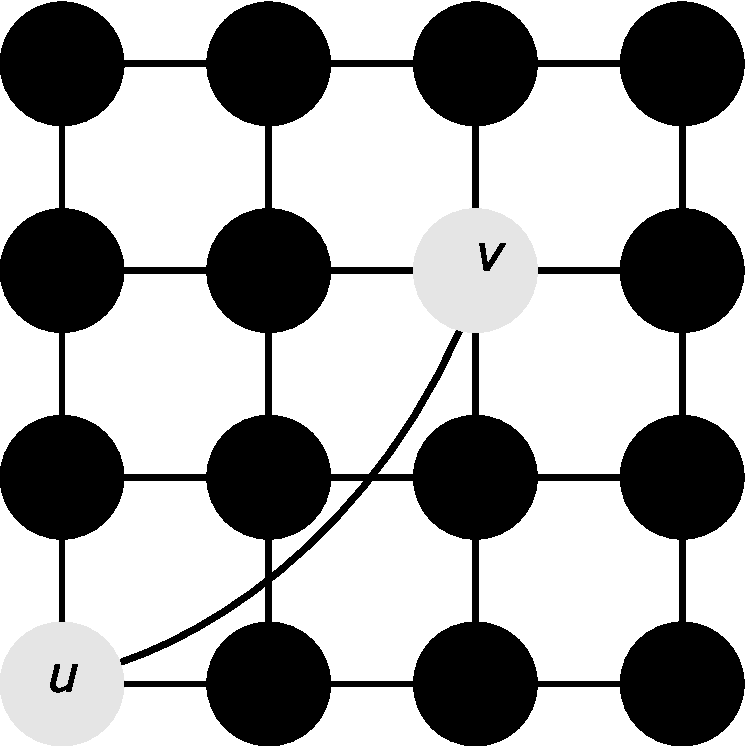
\includegraphics[width=0.25\textwidth]{Grafica/aggregazioniPericolose}} \label{fig:AggA} \quad
\subfloat[][\emph{Due hub connessi. Un hub è un nodo high-degree}.]{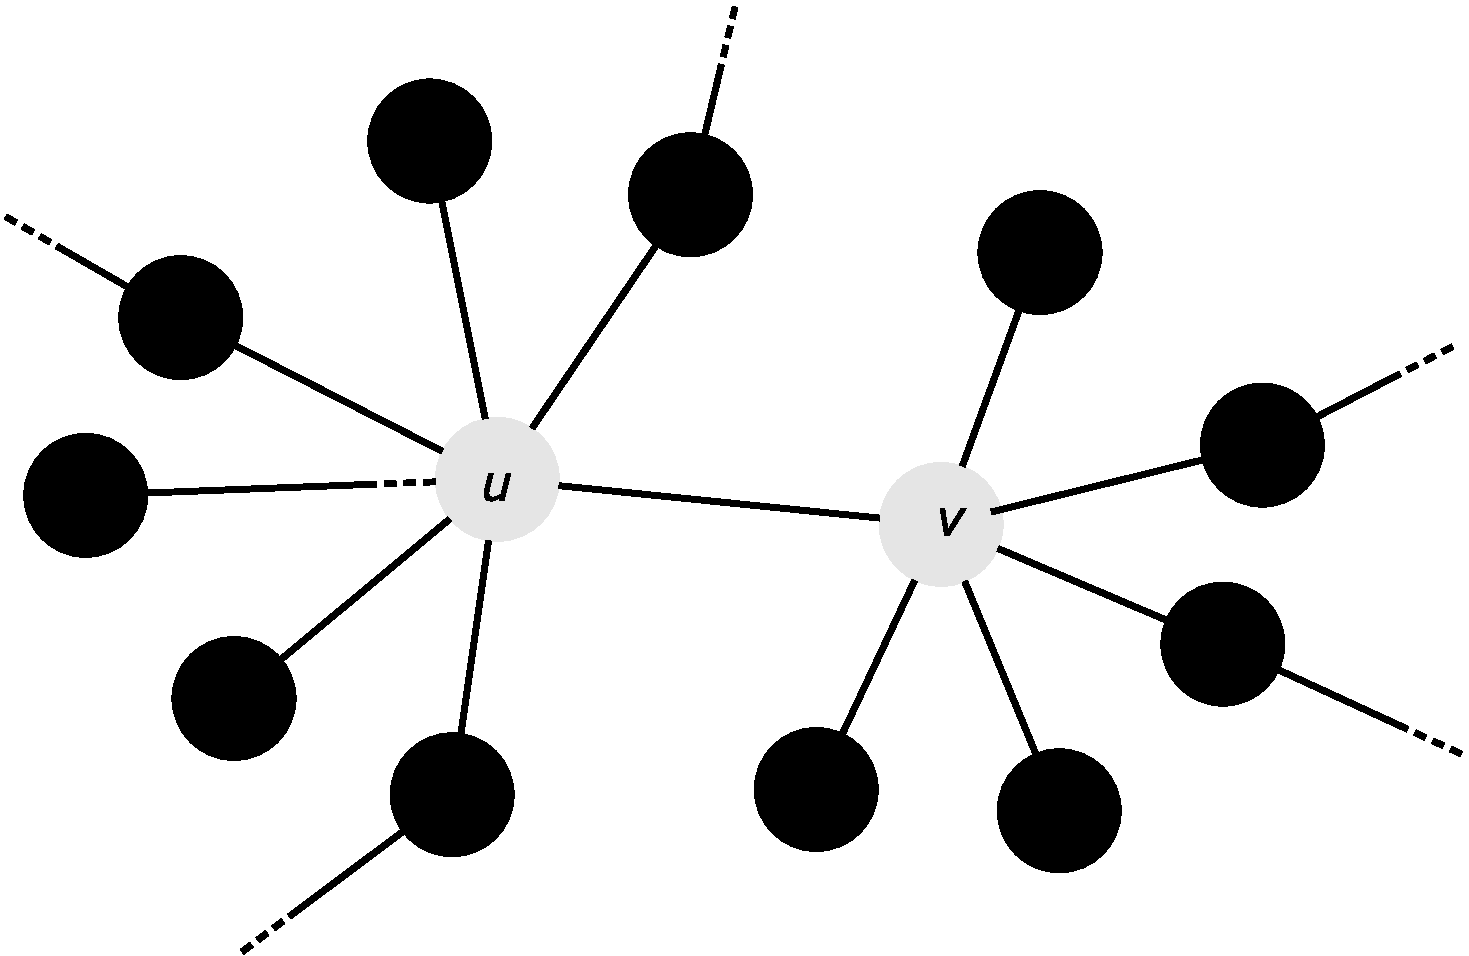
\includegraphics[width=0.35\textwidth]{Grafica/aggregazioniPericolose2}} \label{fig:AggB}\\
\caption{Esempi di aggregazioni pericolose}
\label{fig:Agg}%
\end{figure}%

La misura di prossimità introdotta in LAMG, la \emph{affinity}, gestisce in maniera corretta sia i due casi visti precedentemente sia altri tipi di topologie.
La affinity $c_{uv}$ tra i due nodi $u$ e $v$ è definita come la “bontà'' nell'approssimare  il modello lineare $x_v \approx px_v$ coi valori dei test vector:

\begin{equation}
\label{eqn:Affinity}
c_{uv} = 1 - \frac{ \abs{( X_u, X_v) }^2}{(X_u,X_u)(X_v,X_v)}
\end{equation} 
con $c_{uu} = 0$, $0\le c_{uv} \le 1$ e $c_{uv} = c_{vu}$ e dove
\begin{equation*}
(X,Y) = \sum_{k=1}^K x^{(k)}y^{(k)}
\end{equation*}
mentre 
\begin{equation*}
X_u = (x_u^{(1)}, \dots, x_u^{(K)})
\end{equation*} 

La affinity misura la distanza tra due nodi: più \emph{piccolo} è $c_{uv}$ più \emph{vicini} sono i nodi $u$ e $v$.\\
\\
La creazione di un livello Aggregate equivale a partizionare l'insieme dei nodi $\N$ in $n_c$ sottoinsiemi disgiunti $\{\T_U\}_{U\in\N^c}$, detti \emph{aggregati}.$\T_U$ è l'insieme di $e_u$ interpolato a partire da $e_U^c$ ed $\N^c = \{1,\dots,n_c\}$.
Ogni aggregato consiste in un nodo \emph{seed} e zero o più nodi \emph{associati} (figura~\vref{fig:seeds}).

\begin{figure}%
\centering
\subfloat[][\emph{Il grafo di partenza}.]{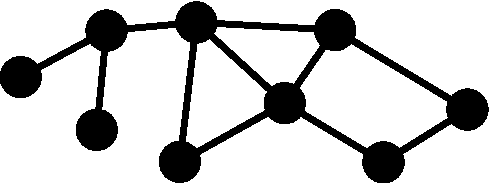
\includegraphics[width=0.25\textwidth]{Grafica/aggr-A}} \quad
\subfloat[][\emph{Una aggregazione. I nodi seed sono indicati in grigio}.]{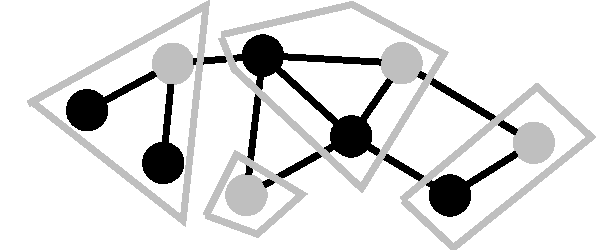
\includegraphics[width=0.25\textwidth]{Grafica/aggr-B}} \\
\subfloat[][\emph{Ciascun aggregato corrisponderà ad un nodo nel grafo coarse}.]{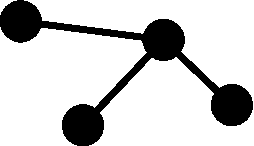
\includegraphics[width=0.20\textwidth]{Grafica/aggr-C}} \\
\caption{Risultati di una aggregazione}
\label{fig:seeds}%
\end{figure}%

Gli aggregati ideali hanno una forte affinity tra di loro, ed una affinity coi rimanenti vicini più debole. 
A tale scopo si definiscono le seguenti regole di aggregazione:

\begin{enumerate}
\item Ogni nodo può essere associato con un solo seed;
\item Un seed può essere associato solo con se stesso;
\item Aggrega prima nodi con affinity minore (più vicini) e poi quelli con affinity maggiore (più lontani);
\item Un nodo hub deve diventare un seed.
\end{enumerate}

Le regole 1-2 hanno lo scopo di evitare associazioni transitive tra seed distanti. Senza di queste si potrebbero creare degli aggregati con connessioni interne deboli tra lunghe catene di seed.
La regola 3 garantisce connessioni locali.
La regola 4, infine, ha lo scopo di evitare decisioni computazionalmente costose derivanti dall'attraversamento del grande insieme di vicini del nodo hub.\\
Un hub è definito come un nodo il cui grado è sufficientemente più alto della media pesata di quello dei suoi vicini:
\begin{equation}
\label{eqn:HubNode}
\abs{\E_u} \ge \frac{ 8\sum_{v\in\E_u} \abs{\w_{uv}}\abs{\E_v} }{ \sum_{v\in\E_u}\abs{\w_{uv}} }
\end{equation}


\begin{algorithm}
\caption{$S = aggregate(\A,\matr{X},\alpha_{\max},I_{\max})$}\label{alg:Aggregate}
\begin{algorithmic}[1]
\State $I_{\max} \gets 2,\, B(1..I_{\max}) \gets \infty,\, n \gets size(\A)$
\State $n_c \gets n,\, \alpha \gets 1,\, i \gets 0,\, \delta \gets 0.9 $
\State $\matr{C} \gets (c_{uv})_{u,v} \text{ where } c_{uv} \gets$ equazione~\eqref{eqn:Affinity} con $\matr{X}$ come test vector, $\forall (u,v) \in \E$
\State For each $u \in \U,\, status(u) \gets \textsc{undecided},\, aggregateSize(u) \gets 1$\label{alg:Aggregate:1}
\State For each $u \in \Set{u : \abs{\E_u} \ge 8\cdot median({\E_v}_v)}, status(u) \gets 0$\label{alg:Aggregate:2}
\While{$(\alpha \ge \alpha_{\max}) \text{ and } (i < I_{\max})$}\Comment{Loop principale di aggregation}
	\State $ i \gets i+1,\, \delta \gets 0.6\delta$
	\State $aggregationStage(status,\A,n_c,\matr{C},\matr{X},aggregateSize,\delta)$
	\State $\alpha \gets n_c/n,\, B_i \gets (1- \alpha \text{ if } \alpha \le \alpha_{\max} \text{ otherwise } 1+ \alpha)$\label{alg:Aggregate:3}
	\State $S_i \gets status$\Comment{Salva l'insieme degli aggregati corrente}
	\State For each $u \in \Set{v:S_i(v) = \textsc{seed}},\,S_i(v) \gets v$
\EndWhile
\State $i \gets \text{argmin}(B)$\Comment{Sceglie il miglior insieme di aggregati}
\State $\text{return } S_i$
\end{algorithmic}
\end{algorithm}


\begin{algorithm}
\caption{$aggregationStage(status,\A,n_c,\matr{C},\matr{X},aggregateSize,\delta)$}\label{alg:aggregationStage}
\begin{algorithmic}[1]
\State $\matr{N} \gets \Set{c_{uv} \ge \delta\cdot\max\Set{\max_{s\ne u} c_{us}, \max_{s\ne v} c_{sv}}} $\Comment{Insieme degli strong neighbors}
\State $\matr{U} \gets \Set{u:status(u) = \text{\textsc{undecided}}}$
\For{each $u \in \matr{U}\cap\Set{u:\E_u\cap\matr{N}} = \emptyset$}\Comment{Nodi undecided con strong neighbors}
	\If{$status(u) \ne \text{\textsc{undecided}}$}\Comment{Lo stato di $u$ può cambiare nel ciclo} 
		\State continue
	\EndIf
	\State $s \gets bestSeed(\A,\matr{X},aggregateSize,\matr{N},\matr{C},u)$
	\If{$s \ne \text{\textsc{notfound}}$}\Comment{$s$ è un seed vicino, aggrega $u$ con $s$}
		\State $status(s)\gets \text{\textsc{seed}},\, status(u) \gets s,\, n_c \gets n_c - 1$
		\State For $k = 1,\dots,K \,,\, x_{uk} \gets x_{sk}$\Comment{Aggiorna i valori del TV}
		\State $aggregateSize(u),aggregateSize(s) \gets aggregateSize(s) + 1$
	\EndIf
\EndFor
\end{algorithmic}
\end{algorithm}

\begin{algorithm}
\caption{$s \gets bestSeed(\A,\matr{X},aggregateSize,\matr{N},\matr{C},u)$}
\label{alg:bestSeed}
\begin{algorithmic}[1]
\State $S \gets \matr{N} \cap \Set{ u : status(u) \in \Set{ \textsc{Undecided}, \textsc{Seed} } }$
\If{$S = \emptyset$}
	\State return \textsc{NotFound}
\Else
	\State return $\argmax{v \in S} c_{uv}$
\EndIf
\end{algorithmic}
\end{algorithm}
L'algoritmo di aggregazio richiede l'indice del ciclo multigrid $\mu$ come parametro di input.
Ogni nodo può essere marcato come \textsc{seed}~(con valore pari a $0$), \textsc{associate}~(con valore pari all'indice del seed a cui è associato) o \textsc{undecided}~(con valore pari a $-1$).

Inizialmente tutti i nodi vengono marcati come \textsc{undecided}~(riga~\ref{alg:Aggregate:1}). 

Si procede poi~(riga~\ref{alg:Aggregate:2}) ad indentificare e marcare come seed tutti i nodi hub utilizzando la formula~\eqref{eqn:HubNode}.

Poi si scartano gli archi che hanno un peso $\abs{\w_{uv}}$ molto piccolo per accelerare la velocità di convergenza è ridurre il numero di calcoli da effettuare.

I nodi che eventualmente divengono disconnessi vengono aggregati insieme in un unico seed fittizio al fine di mantenere la matrice una Laplaciana.
I rimanenti nodi vengono marcati come \textsc{undecided}.

L'aggregazione vera e propria avviene in $r$ stage. Si generano $S_1,\dots,S_i,\dots,S_r$ insiemi aggregati tali che ogni aggregato $S_i$ sia contenuto in alcuni aggregati $S_{i+1}$.
L'insieme per cui il fattore di coarsening $\alpha = \abs{S_i}/n$ è più vicino ad $\alpha_{\max} = 0.7 / \mu$ viene scelto come insieme finale. 

Nel codice vengono effettuati al più \emph{due} stage di aggregazione per ogni livello di coarsening nel ciclo.

In ognuna di queste stage si scorrono i nodi undecided $u$ e si procede ad aggregare ognuno di questi con un suo vicino $s$ che può essere un nodo già marcato come \textsc{seed} oppure un altro nodo \textsc{undecided}, che dunque diviene un nuovo seed.

Per effettuare tale decisione, riassunta dall'algoritmo~\vref{alg:bestSeed}, si utilizza la affinity.

L'algoritmo~\vref{alg:aggregationStage} riassume il comportamento di uno stage di aggregazione, l'algoritmo~\vref{alg:Aggregate} un'intera procedura di aggregazione.


\sezione{L'algoritmo di LAMG}

\sottosezione{Fase di setup}
\label{faseSetup}

Il solo dato di input è il parametro $\mu \geq 1$ che determina l'andamento del ciclo multigrid.
Il problema originale, corrispondente al livello $l = 1$ viene ripetutamente \emph{coarsened} utilizzando l'eliminazione o l'aggregazione lineare fino a che il numero di nodi non scende sotto i $150$ o finché il rilassamento non converge rapidamente.
Si utilizzano $K=4$ test vector per i livelli più fini; questo numero viene aumentato per i livelli più coarse fino ad un massimo di $10$. Ciascun test vector viene ammorbidito utilizzando $\nu = 3$ passaggi di rilassamento del metodo di Gauss-Seidel.

\sottosezione{Fase di solve}
La fase di solve consiste in cicli multigrid del tutto simili a quelli descritti dall'algoritmo~\vref{alg:MGM}.
A ciascun livello $l < L$ viene assegnato un indice di ciclo $\mu^l$ e due indici $\nu_{pre}^l$ ed $\nu_{post}^l$ che indicano il numero di pre- e post- rilassamenti da effettuare sull'errore.
Se il livello $l+1$ è il risultato di una eliminazione allora $\mu^l = 1$ e $\nu_{pre}^l = \nu_{post}^l = 0$ altrimenti:
\begin{equation}
\mu^l = 
\begin{cases}
1 & \text{se } |\E^l| > 0.1|\E|\\
\min\{2,0.7 |\E^{l+1}| / |\E^l|\} & \text{ altrimenti}
\end{cases},\quad
\nu_{pre}^l = 1,\, \nu_{post}^l=2
\end{equation}